\documentclass{beamer}
\usetheme{Boadilla}
\usepackage{tikz}
 \usepackage[english]{babel}
 \usepackage{amsmath}
 \usepackage{amssymb}
 \usepackage{amsthm}
 \usepackage{mathtools} 
 \usepackage[utf8]{inputenc}
 \usepackage{dsfont}
 \usetikzlibrary{patterns}
 \usepackage{mathrsfs}
 \usepackage{ bbold }
\usetikzlibrary{mindmap,trees,shadows}
\usepackage{caption}
\usepackage{tabularx}
\usepackage{booktabs}
% \usepackage{apacite}
\usepackage{listings}
\captionsetup[figure]{font=scriptsize}
\newcommand{\MYhref}[3][blue]{\href{#2}{\color{#1}{#3}}}%
\usepackage{hyperref} 
            \hypersetup{backref=true,       
                    pagebackref=true,               
                    hyperindex=true,                
                    colorlinks=true,                
                    breaklinks=true,                
                    urlcolor= blue,                
                    linkcolor= blue,                
                    bookmarks=true,                 
                    bookmarksopen=false,
                    citecolor=blue,
                    linkcolor=blue,
                    filecolor=blue,
                    citecolor=blue,
                    linkbordercolor=blue
}

\definecolor{background}{RGB}{39, 40, 34}
\definecolor{string}{RGB}{230, 219, 116}
\definecolor{comment}{RGB}{117, 113, 94}
\definecolor{normal}{RGB}{248, 248, 242}
\definecolor{identifier}{RGB}{166, 226, 46}

\lstset{
  language = SQL,  % choose the language of the code
  linewidth = 12cm,
  numbers = left, % where to put the line-numbers
  stepnumber=1,  % the step between two line-numbers.
  numbersep=5pt, % how far the line-numbers are from the code
  numberstyle=\tiny\color{black}\ttfamily,
  backgroundcolor=\color{background}, % choose the background color. You must add \usepackage{color}
  showspaces=false, % show spaces adding particular underscores
  showstringspaces=false,             % underline spaces within strings
  showtabs=false, % show tabs within strings adding particular underscores
  tabsize=4,                          % sets default tabsize to 2 spaces
  captionpos=b,                       % sets the caption-position to bottom
  breaklines=true,                    % sets automatic line breaking
  breakatwhitespace=true, % sets if automatic breaks should only happen at whitespace
  title=\lstname,  % show the filename of files included with \lstinputlisting;
  basicstyle=\color{normal}\ttfamily,     % sets font style for the code
  keywordstyle=\color{magenta}\ttfamily,  % sets color for keywords
  stringstyle=\color{string}\ttfamily,    % sets color for strings
  commentstyle=\color{comment}\ttfamily,  % sets color for comments
  emph={format_string, eff_ana_bf, permute, eff_ana_btr},
  emphstyle=\color{identifier}\ttfamily,
  belowskip=-0.5cm
}

\title[High Dimensional Models] % (optional, only for long titles)
{High Dimensional Models}
\subtitle{Time-Varying Graphical Lasso}
\author[Andrew Boomer \& Jacob Pichelmann] % (optional, for multiple authors)
{Andrew Boomer \& Jacob Pichelmann}
\institute []
{Toulouse School of Economics \\ M2 EEE}

\date{\today}

\usepackage[backend=biber]{biblatex}
\bibliography{References.bib}
\usepackage{csquotes}
\RequirePackage{filecontents}

\begin{document}


\frame{\titlepage}
    
\begin{frame}{Introduction to Graphs}
    \begin{itemize}
        \item A graph is represented by a set of vertices $V = \{1, 2, \dotsb, p\}$ and by a set of edges $E \subset V x V$
        \item A graph is undirected when there is no distinction between the edge $(s, t)$ and $(t, s) \quad \forall \ s, t \in E$
        \item Graphs can also be thought of in terms of Markov chains, and some of the properties and representations of Markov Chains apply to graphs as well
        \item For example, the edge set of a graph can be represented as a Markov transition matrix. For an edge set $E \subset (a, b) x (a, b)$ the matrix would be:
        \[\begin{bmatrix} W_{(a, a)} & W_{(a, b)} \\
           W_{(b, a)} & W_{(b, b)} \end{bmatrix}\]
    \end{itemize}
\end{frame}

\begin{frame}{Extension to Graphical Models}
  \begin{itemize}
    \item This graphical representation can be extended to a high dimensional set of random variables $X_{s}$.
    \item In this example, $s$ corresponds to a single vertex with the whole vertex set $V$ of the total graph. The connections between each vertex in the Markov transition matrix representation quanity the relationship between this random variables.
  \end{itemize}
  \begin{figure}
  \begin{minipage}{0.4\textwidth}
      The two in Figure \ref{fig:IntroPic} are equivalent, where white spaces indicate no relationship, and grey spaces indicate a 1-to-1 relationship.
  \end{minipage}%
  \begin{minipage}{0.6\textwidth}
    \begin{figure}
       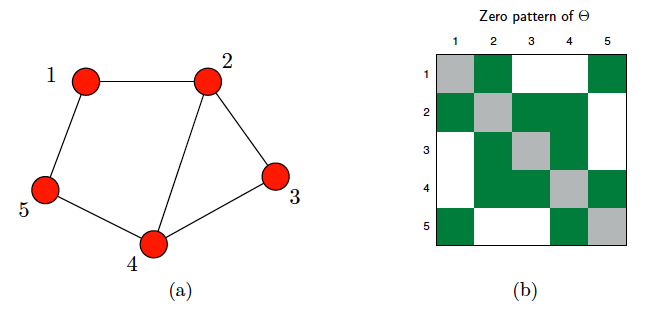
\includegraphics[width=6cm]{IntroGraphMat.png}
       \caption{Graph and Sparsity Matrix}
       \label{fig:IntroPic}
  \end{figure} 
  \end{minipage}
  \end{figure}
\end{frame}

\begin{frame}{Gaussian Graphical Models}
  \begin{itemize}
    \item For a guassian graphical model, we start from a gaussian distribution with dimension equal to the number of vertices $X \sim \mathcal{N}(\mu, \Sigma)$
    \item The sparsity matrix in the slide above, for a gaussian graphical model, is given by $\Theta = \Sigma^{-1}$, and is also known as the precision matrix. The goal of a gaussian graphical model is to solve for $\Theta$.
    \item The gaussian distribution can be rewritten in terms of a maximum likelihood problem to solve for $\hat{\Theta}_{MLE}$, where $S$ is the empirical covariance matrix, rearranged and simplified to:
    \[\mathcal{L}(\Theta; X) = log \ det \ \Theta - trace(S \Theta)\]
    \item This MLE problem converges to the true precision matrix when $N \xrightarrow{} \infty$. The MLE problem is, however, not even feasible if $p > N$, where $p$ is the number of dimensions.
  \end{itemize}
\end{frame}

\begin{frame}{Graphical LASSO}
  \begin{itemize}
    \item As with a regression LASSO, adding a regularization term solves the issue of a non-full rank matrix. Additionally, the LASSO term induces low-importance terms to zero.
    \item In the case of the graphical LASSO, weak edge connections in the precision matrix will go to zero, increasing the sparsity of the resulting solution.
    \item Whereas in the regression LASSO, large values of the $\beta$ parameter were penalized, in the graphical LASSO, large values in the off-diagonal entries of the precision matrix will be penalized.
    \item Where $\lambda$ is the LASSO penalty and $p_{1}(\Theta) = \sum_{s \neq t} |\theta_{st}|$, The maximization problem is:
    \[\hat{\Theta} \in argmax \{log \ det \ \Theta - trace(S\Theta) - \lambda p_{1}(\Theta)\}\]
  \end{itemize}
\end{frame}

\begin{frame}{Time Varying Graphical LASSO}
  \begin{itemize}
    \item In their paper \cite{hallac2017network}, the authors discuss a method to estimate the change in a network's structure over time. This is accomplished with the addition of another parameter to penalize the change in network structure over time. The time-varying maximization problem is:
    \[\hat{\Theta}_{T} \in argmax \{log \ det \ \Theta - trace(S\Theta) - \lambda p_{1}(\Theta) - \beta \sum_{t = 2}^{T} \psi(\Theta_{t} - \Theta_{t - 1}\}\]
    \item Here, $\psi$ is a convex function which encourages similarity between $\Theta_{t}$ and $\Theta_{t - 1}$. Different choices of $\psi$ can penalize different changes in network structure.
  \end{itemize}
\end{frame}

\begin{frame}{Time Penalty Functions}
  The authors lay out 5 different choices for the function $\psi$ in \cite{hallac2017network}.
  \begin{enumerate}
    \item \textbf{A few edges changing at a time:} $\psi(X) = \sum_{i, j} |X_{ij}|$
    \item \textbf{Global Restructuring:} $\psi(X) = \sum_{j} ||[X]_{j}||_{2}$
    \item \textbf{Smoothly Varying Over Time:} $\psi(X) = \sum_{i, j} X_{ij}^{2}$
  \end{enumerate}
\end{frame}

\begin{frame}
  \nocite{*}
  \printbibliography
\end{frame}

\end{document}